\documentclass[a4paper, 12pt]{report}		% general format

%%%% Charset
\usepackage{cmap}							% make PDF files searchable and copyable
\usepackage[utf8]{inputenc}					% accept different input encodings
\usepackage[T2A]{fontenc}					% russian font
\usepackage[russian]{babel}					% multilingual support (T2A)

%%%% Graphics
\usepackage[dvipsnames]{xcolor}			% driver-independent color extensions
\usepackage{graphicx}						% enhanced support for graphics
\usepackage{wrapfig}						% pro­duces fig­ures which text can flow around

%%%% Math
\usepackage{amsmath}						% Amer­i­can Math­e­mat­i­cal So­ci­ety (AMS) math fa­cil­i­ties
\usepackage{amsfonts}						% fonts from the AMS
\usepackage{amssymb}						% additional math symbols

%%%% Ty­po­grapy (don't forget about cm-super)
\usepackage{microtype}						% sublim­i­nal re­fine­ments to­wards ty­po­graph­i­cal per­fec­tion
\linespread{1.3}							% line spacing
\usepackage[left=2.5cm, right=1.5cm, top=2.5cm, bottom=2.5cm]{geometry}
\setlength{\parindent}{0pt}					% we don't want any paragraph indentation
\renewcommand{\chaptername}{}

%%%% Other
\usepackage{url}							% ver­ba­tim with URL-sen­si­tive line breaks
%\DeclareUnicodeCharacter{00A0}{~}

%------------------------------------------------------------------------------
\usepackage{listings}						% type­set source code list­ings

% Цвета для кода
\definecolor{string}{HTML}{101AF9}			% цвет строк в коде
\definecolor{comment}{HTML}{0C2612}		% цвет комментариев в коде
\definecolor{keyword}{HTML}{5F1441}		% цвет ключевых слов в коде
\definecolor{morecomment}{HTML}{8000FF}	% цвет include и других элементов в коде
\definecolor{captiontext}{HTML}{FFFFFF}	% цвет текста заголовка в коде
\definecolor{captionbk}{HTML}{999999}		% цвет фона заголовка в коде
\definecolor{bk}{HTML}{FFFFFF}				% цвет фона в коде
\definecolor{frame}{HTML}{999999}			% цвет рамки в коде

% Настройки отображения кода
\lstset{
	language=C++,							% Язык кода по умолчанию
	morekeywords={*,...},					% если хотите добавить ключевые слова, то добавляйте
	% Цвета
	keywordstyle=\color{keyword}\ttfamily\bfseries,
	stringstyle=\color{string}\ttfamily,
	commentstyle=\color{comment}\ttfamily\itshape,
	morecomment=[l][\color{morecomment}]{\#},
	% Настройки отображения
	breaklines=true,						% Перенос длинных строк
	basicstyle=\ttfamily\footnotesize,		% Шрифт для отображения кода
	backgroundcolor=\color{bk},				% Цвет фона кода
	%frame=lrb,xleftmargin=\fboxsep,xrightmargin=-\fboxsep, % Рамка, подогнанная к заголовку
	frame=tblr								% draw a frame at all sides of the code block
	rulecolor=\color{frame},				% Цвет рамки
	tabsize=2,								% tab space width
	showstringspaces=false,					% don't mark spaces in strings
	% Настройка отображения номеров строк. Если не нужно, то удалите весь блок
	numbers=left,							% Слева отображаются номера строк
	stepnumber=1,							% Каждую строку нумеровать
	numbersep=5pt,							% Отступ от кода
	numberstyle=\small\color{black},		% Стиль написания номеров строк
	% Для отображения русского языка
	extendedchars=true,
	literate={Ö}{{\"O}}1
	 	{Ä}{{\"A}}1
	 	{Ü}{{\"U}}1
		{ß}{{\ss}}1
		{ü}{{\"u}}1
		{ä}{{\"a}}1
		{ö}{{\"o}}1
		{~}{{\textasciitilde}}1
		{а}{{\selectfont\char224}}1
		{б}{{\selectfont\char225}}1
		{в}{{\selectfont\char226}}1
		{г}{{\selectfont\char227}}1
		{д}{{\selectfont\char228}}1
		{е}{{\selectfont\char229}}1
		{ё}{{\"e}}1
		{ж}{{\selectfont\char230}}1
		{з}{{\selectfont\char231}}1
		{и}{{\selectfont\char232}}1
		{й}{{\selectfont\char233}}1
		{к}{{\selectfont\char234}}1
		{л}{{\selectfont\char235}}1
		{м}{{\selectfont\char236}}1
		{н}{{\selectfont\char237}}1
		{о}{{\selectfont\char238}}1
		{п}{{\selectfont\char239}}1
		{р}{{\selectfont\char240}}1
		{с}{{\selectfont\char241}}1
		{т}{{\selectfont\char242}}1
		{у}{{\selectfont\char243}}1
		{ф}{{\selectfont\char244}}1
		{х}{{\selectfont\char245}}1
		{ц}{{\selectfont\char246}}1
		{ч}{{\selectfont\char247}}1
		{ш}{{\selectfont\char248}}1
		{щ}{{\selectfont\char249}}1
		{ъ}{{\selectfont\char250}}1
		{ы}{{\selectfont\char251}}1
		{ь}{{\selectfont\char252}}1
		{э}{{\selectfont\char253}}1
		{ю}{{\selectfont\char254}}1
		{я}{{\selectfont\char255}}1
		{А}{{\selectfont\char192}}1
		{Б}{{\selectfont\char193}}1
		{В}{{\selectfont\char194}}1
		{Г}{{\selectfont\char195}}1
		{Д}{{\selectfont\char196}}1
		{Е}{{\selectfont\char197}}1
		{Ё}{{\"E}}1
		{Ж}{{\selectfont\char198}}1
		{З}{{\selectfont\char199}}1
		{И}{{\selectfont\char200}}1
		{Й}{{\selectfont\char201}}1
		{К}{{\selectfont\char202}}1
		{Л}{{\selectfont\char203}}1
		{М}{{\selectfont\char204}}1
		{Н}{{\selectfont\char205}}1
		{О}{{\selectfont\char206}}1
		{П}{{\selectfont\char207}}1
		{Р}{{\selectfont\char208}}1
		{С}{{\selectfont\char209}}1
		{Т}{{\selectfont\char210}}1
		{У}{{\selectfont\char211}}1
		{Ф}{{\selectfont\char212}}1
		{Х}{{\selectfont\char213}}1
		{Ц}{{\selectfont\char214}}1
		{Ч}{{\selectfont\char215}}1
		{Ш}{{\selectfont\char216}}1
		{Щ}{{\selectfont\char217}}1
		{Ъ}{{\selectfont\char218}}1
		{Ы}{{\selectfont\char219}}1
		{Ь}{{\selectfont\char220}}1
		{Э}{{\selectfont\char221}}1
		{Ю}{{\selectfont\char222}}1
		{Я}{{\selectfont\char223}}1
		{і}{{\selectfont\char105}}1
		{ї}{{\selectfont\char168}}1
		{є}{{\selectfont\char185}}1
		{ґ}{{\selectfont\char160}}1
		{І}{{\selectfont\char73}}1
		{Ї}{{\selectfont\char136}}1
		{Є}{{\selectfont\char153}}1
		{Ґ}{{\selectfont\char128}}1
}

% Для настройки заголовка кода
\usepackage{caption}
\DeclareCaptionFont{white}{\color{сaptiontext}}
\DeclareCaptionFormat{listing}{\parbox{\linewidth}{\colorbox{сaptionbk}{\parbox{\linewidth}{#1#2#3}}\vskip-4pt}}
%\captionsetup[lstlisting]{format=listing,labelfont=white,textfont=white}
\renewcommand{\lstlistingname}{Листинг} % Переименование Listings в нужное именование структуры

%------------------------------------------------------------------------------
\begin{document}

\begin{titlepage}
\thispagestyle{empty}

\begin{center}
Санкт-Петербургский государственный политехнический университет \\
Институт Информационных Технологий и Управления \\*
Кафедра компьютерных систем и программных технологий \\*
\hrulefill
\end{center}

\vspace{18em}

\begin{center}
\Large Отчет по лабораторным работам \\ по предмету "Параллельные вычисления" \\
\end{center}

\vspace{1em}

% \linebreak
\begin{center}
\textsc{\textbf{Параллельная обработка Б-деревьев}}
\end{center}

\vspace{16em}

\begin{flushleft}
Работу выполнил студент гр. 53501/3\hrulefill Мартынов С. А. \\
\vspace{1.5em}
Работу принял преподаватель \hrulefill Моисеев М.Ю. \\
\end{flushleft}

\vspace{\fill}

\begin{center}
Санкт-Петербург \\
2014
\end{center}

\end{titlepage}
%------------------------------------------------
\setcounter{page}{2}
\tableofcontents
%------------------------------------------------

\chapter*{Введение}
\addcontentsline{toc}{chapter}{Введение}

В последнее время тактовая частота центральных процессоров прекратила бурный рост, который наблюдался в последние десятилетия и производители сосредоточились на увеличении количества ядер. Это открыло новые возможности для разработчиков, т.к. позволило увеличить производительность программ не прибегая к механическому вертикальному масштабированию.
\vspace{1em}

Воспользоваться преимуществами нескольких ядер относительно просто для серверных приложений, где каждый поток может независимо обрабатывать отдельный запрос от клиента, но этого значительно сложнее добиться для клиентских приложений, поскольку в этом случае обычно потребуется преобразовать код, интенсивно использующий вычисления и средства межпроцессной и межпоселковой синхронизации.
\vspace{1em}

В данной работе рассмотрена работа со следующими инструментами:

\begin{enumerate}
    \item Pthtreads;
    \item OpenMP;
    \item C++11.
\end{enumerate}

В качестве задачи было принято решение реализовать поточную обработку B-дерева, часто применяемого в базах данных.

\vspace{1em}
Исходный код всех представленных листингов доступен по адресу \\ \url{https://github.com/SemenMartynov/SPbPU_ParallelProgramming}.

%------------------------------------------------

\chapter*{Реализация однопоточного алгоритма}
\addcontentsline{toc}{chapter}{Реализация однопоточного алгоритма}

Для начала была реализована однопоточная версия. Она состоит из двух классов BTree и BTreeNode. Заголовочные файлы этих классов представлены в листинге 1 и листинге 2. Реализацию можно изучить на гитхабе, ссылка была приведена во введении.

\lstinputlisting[language=C++, caption={заголовочный файл класса BTree}]
{../tests/BTree.h}

\lstinputlisting[language=C++, caption={заголовочный файл класса BTreeNode}]
{../tests/BTreeNode.h}

Корректность кода проверялась при помощи Google test framework (смотри листинг 3) и valgrind (смотри изображение 1).

\lstinputlisting[language={},caption={Лог тестирование программы при помощи Google test framework}]{res/test.log}

\begin{figure}[h!]
\centering
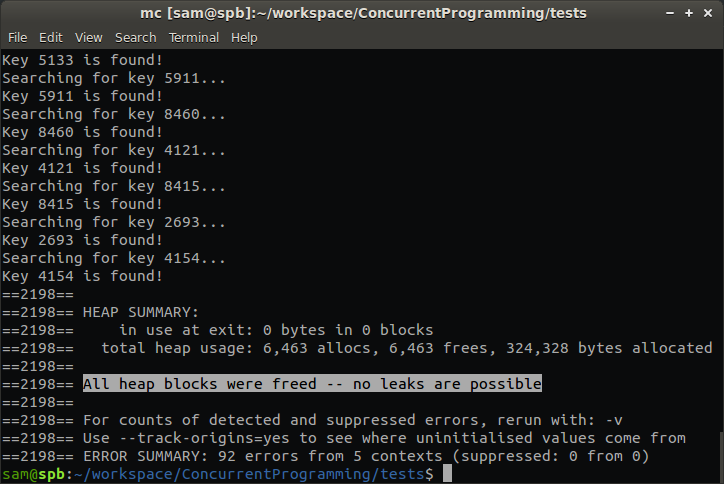
\includegraphics[scale=0.68]{res/valgrind}
\caption{Поиск утечек памяти при помощи valgrind}
\end{figure}

%------------------------------------------------

\chapter*{Многопоточные программирование с использованием Pthreads}
\addcontentsline{toc}{chapter}{Многопоточные программирование с использованием Pthreads}

В той или иной форме, библиотека Pthread представлена на всех современных операционных системах. Она предоставляет низкоуровневый механизм управления процессами что даёт большую производительность но и требует больших трудозатрат. В листинге 4 один поток пополняет дерево, один удаляет элементы, и ещё несколько осуществляют поиск по дереву.

\lstinputlisting[language=C++, caption={Работа с B-деревом при помощи Pthreads}]
{../pthreads/main.cpp}

%------------------------------------------------

\chapter*{Многопоточные программирование с использованием OpenMP}
\addcontentsline{toc}{chapter}{Многопоточные программирование с использованием OpenMP}

Наиболее удобным средством для быстрого распараллеливания уже написанного кода является OpenMP. С другой стороны, его сложнее отлаживать и контролировать. К тому же, не являясь частью языка или библиотеки, OpenMP не поддерживается некоторыми статическими анализаторами на этапе разработки, что тоже создаёт неудобства. На листинге 5 представлена реализация задачи построения B-дерева с использованием OpenMP.

\lstinputlisting[language=C++, caption={Работа с B-деревом из OpenMP}]
{../openmp/main.cpp}

%------------------------------------------------

\chapter*{Многопоточные программирование с использованием С++11}
\addcontentsline{toc}{chapter}{Многопоточные программирование с использованием С++11}

Представленный в 2011-м году стандарт языка C++ получил поддержку потоков. По сути, это более высокоуровневая абстракция над библиотекой Pthreads, но работать становится на много приятнее за счёт использования таких механизмов как лямбды. Код в итоге получается удобно читаемым и компактным. На листинге 6 представлена работа с C++11.

\lstinputlisting[language=C++, caption={Потоки C++11}]
{../cpp11/main.cpp}

%------------------------------------------------

\chapter*{Многопроцессные приложения c POSIX синхронизацией}
\addcontentsline{toc}{chapter}{Многопроцессные приложения c POSIX синхронизацией}

В этой программе используется семафор, вмещающий 4 потребителя. При этом в программе создаётся 6 процессов (средствами вызова fork()) и основной процесс. Дочерние процессы проверяют наличие ключа в дереве, а родительский постепенно уничтожает эти ключи. Каждый дочерний процесс работает какое-то время, которое определяется генератором случайных чисел. Код, реализующий эту идею, представлен в листинге 7.

\lstinputlisting[language=C++, caption={Синхронизация средствами POSIX}]
{../IPC/main.cpp}


%------------------------------------------------

\chapter*{Заключение}
\addcontentsline{toc}{chapter}{Заключение}

Многопоточность является естественным продолжением многозадачности, точно также как виртуальные машины, позволяющие запускать несколько ОС на одном компьютере, представляют собой логическое развитие концепции разделения ресурсов.
\vspace{1em}

Уровень контроля над потоками в многопоточном приложении выше, чем уровень контроля приложения над дочерними процессами. Кроме того, многопоточные программы не склонны оставлять за собой вереницы зомби или «осиротевших» независимых процессов. Для отслеживания подобных ситуаций можно использовать специальный отладчики и средства, предоставляемые операционной системой.
\vspace{1em}

Из инструментов, рассмотренных в данной работе наилучшее впечатление оставил о себе C++11. В C++11, работа с потокам осуществляется по средствам класса std::thread (доступного из заголовочного файла <thread>), который может работать с регулярными функциями, лямбдами и функторами. В данной работе не покрыты все возможности языка, вопрос требует дополнительного изучения.

%------------------------------------------------

\chapter*{Список литературы}
\addcontentsline{toc}{chapter}{Список литературы}

\begin{enumerate}
    \item Х.М. Дейтел,П.Дж. Дейтел, Д.Р. Чофнес. Операционные системы: Основы и принципы. Третье     \item издание. Пер. с англ. - М.ООО"Бинм-Пресс", 2009 г. - 1024 с.
    \item Воеводин В. В., Воеводин Вл. В. Параллельные вычисления — СПб: БХВ-Петербург, 2002. — 608 с.
    \item Немнюгин С., Стесик О. - Параллельное программирование для многопроцессорных вычислительных систем. - СПб. БХВ-Петербург,2002. – 400с.
    \item Робачевский А., Немнюгин С., Стесик О. - Операционная система UNIX, 2 изд., СПб: БХВ 2010.- 656c.
    \item Боресков А.В., Харламов А.А. Основы работы с технологией CUDA. М:ДМК-Пресс. 2010, -232с.
    \item B. Nichols, D. Buttlar, J.P. Farrell: Pthreads Programming - A POSIX Standard for Better Multiprocessing, O'Reilly, 1996.-288p.
    \item B. Eckel. Thinking in Java (4th Edition). Prentice Hall, 2006.-1150p.
    \item B. Goetiz, T. Peierls. Java concurrency in practice. Addison-Wesley Professional, 2006, - 384p.
    \item IEEE standard SystemC language reference manual, IEEE Std 1666, 2005\\ – http://standards.ieee.org/getieee/1666/download/1666-2005.pdf
    \item Официальный сайт OpenMP – http://openmp.org/wp/
    \item Message Passing Interface Forum – http://www.mpi-forum.org/
\end{enumerate}

\end{document}
